%!TEX root = ../../main.tex

\emph{Deep Learning} (DL), também conhecido como Aprendizado Profundo, é uma subárea específica de AM que enfatiza o aprendizado através de sucessivas camadas de representações cada vez mais significativas dos dados submetidos. No caso das redes neurais, tais representações são obtidas pelas camadas profundas \cite{chollet}, isto é, pelas camadas ocultas que ocorrem em maior número do que nas redes neurais rasas, como as \emph{multilayer perceptron}, comumente contendo mais que duas camadas ocultas \cite{heaton}. A utilização de DL tem obtido êxito em endereçar problemas de Visão Computacional e Processamento de Linguagem Natural. Estes algoritmos não só ultrapassaram o desempenho de outras variedades de algoritmos de AM, como também pleiteam a eficácia na classificação alcançada por seres humanos \cite{buduma}.

Os motivos para o corrente sucesso do DL podem ser exemplificados pela grande quantidade de dados disponíveis -- como a base de dados \emph{ImageNet}, organizada conforme a hierarquia \emph{WordNet} e que disponibiliza imagens para pesquisadores ao redor do mundo \cite{imagenet} -- e o custo relativamente baixo de Unidades de Processamento Gráfico (GPUs), que são utilizadas para uma computação numérica muito mais eficiente. Grandes companhias do ramo tecnológico utilizam técnicas de DL diariamente para a análise de enormes quantidades de dados. Entretanto, esta especiliadade não é mais limitada somente ao domínio acadêmico e industrial, ela tornou-se parte integrante da produção de softwares modernos disponibilizados aos consumidores \cite{gulli}.

\todo{Adicionar um parágrafo com exemplos de soluções com Deep Learning. Trabalho da Nicoli, do Sérgio, Janderson, e outros.}

O ferramental de DL compreende um conjunto de técnicas e modelos que podem ser aplicados a tarefas de aprendizado supervisionado e não-supervisionado. Porém, dentre os diferentes modelos existentes, as redes neurais convolucionais se destacam expressivamente, com um bom desempenho em diversos tipos de tarefas. A próxima seção descreve os pontos principais relacionados a este tipo de modelo.

\subsubsection{Redes Neurais Convolucionais}
\label{subsubsec:cnns}

As \emph{Redes Neurais Convolucionais} (CNNs, do inglês \emph{Convolutional Neural Networks}) são uma categoria de redes neurais profundas, \emph{feedforward}, que comprovaram ser extremamente bem-sucedidas no ramo de visão computacional \cite{khan}. O termo denominado a estas redes, vem do seu aproveitamento da operação matemática chamada convolução, um tipo especializado de operação linear \cite{goodfellow}. Na Figura \ref{fig:areas-ia} é ilustrada a relação das CNNs com alguns campos de estudos conhecidos.

\begin{figure}[h!]
  \centering
  \caption{A relação entre a visão humana, visão computacional, AM, DL e CNNs. Adaptado de: \cite{khan}.}
  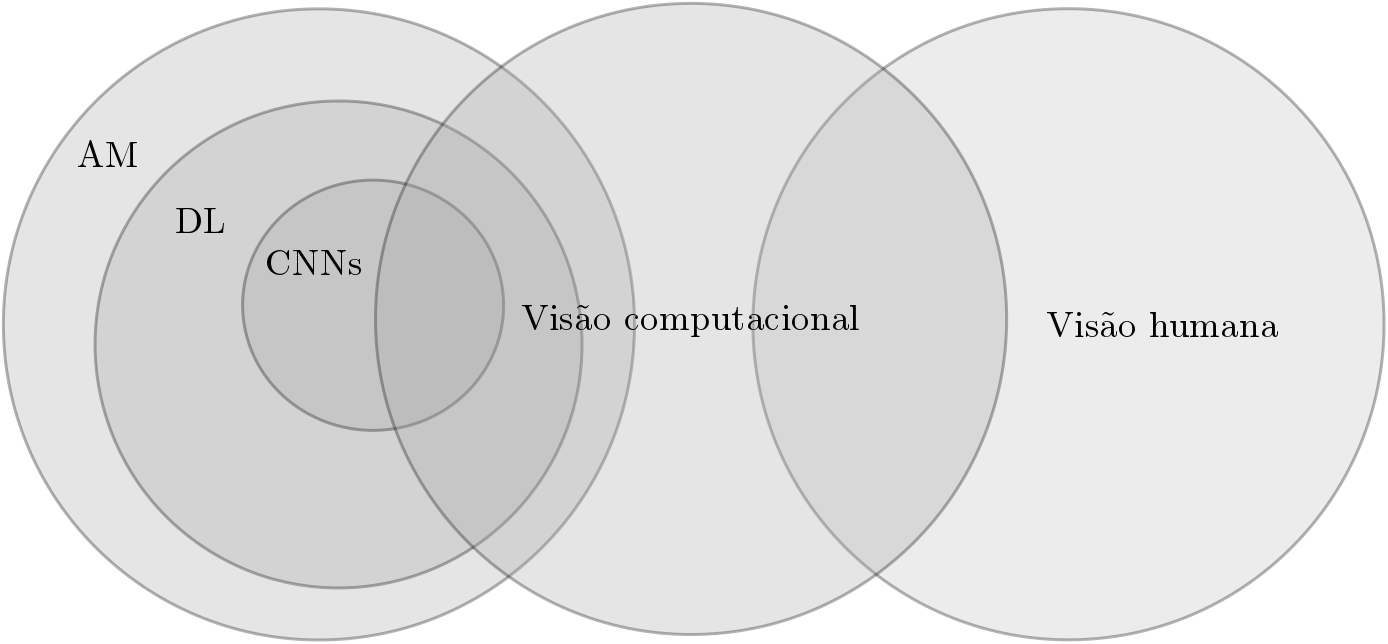
\includegraphics[width=0.7\textwidth]{imgs/areas-ia}
  \label{fig:areas-ia}
\end{figure}

% Convolução
\added{Para caracterizar as CNNs, é necessário conceituar as suas partes integrantes, em especial, as noções de convolução, \emph{pooling}, as camadas completamente conectadas, operações de \emph{droupout}, dentre outras.}
A \emph{convolução}, em especial, é uma operação que consiste na soma dos produtos de toda a extensão de duas entradas em função de um deslocamento. Sendo assim, a convolução $s(t)$ de duas entradas $x_1(t)$ e $x_2(t)$ é uma função representada simbolicamente por $s(t) = x_1(t) * x_2(t)$ é definida conforme a Equação \ref{eq:conv} \cite{lathi}.

\begin{equation}
  \label{eq:conv}
  s(t) = x_1(t) * x_2(t) = \int_{-\infty}^{\infty} x_1(\tau)x_2(t - \tau)d\tau
\end{equation}

Nas aplicações de AM, a função $x_1(t)$ é chamada de \emph{input}, a função $x_2(t)$ é o \emph{filtro}, também conhecido como \emph{kernel}, e a saída $s(t)$ consiste no \emph{mapa de características}, gerado pela convolução. O \emph{input} é geralmente uma matriz multidimensional de dados de entrada e o filtro é uma matriz multidimensional de de parâmetros que são ajustados pelo algoritmo de aprendizado. Uma matriz multidimensional no contexto de AM é comumente referenciada como \emph{tensor} \cite{goodfellow}.

Nas CNNs, as camadas convolucionais são responsáveis por aplicar as operações de convolução. Tomando como exemplo um problema de reconhecimento de padrões em uma imagem, cada camada é responsável por desenvolver os atributos detectados nas camadas anteriores -- de linhas, a contornos, a formatos, até construir um objeto por completo. Esse processo pode ser visualizado na Figura \ref{fig:camadas-convolucionais}. \replaced{O trecho a seguir não está claro. Precisa redigir melhor}{Nestas camadas, os mapas de características são capturados, e nestes consistem os pesos da rede que são responsáveis por identificar onde são encontrados os atributos na imagem original \cite{buduma}.}

\begin{figure}[h!]
\centering
\caption{Exemplo de processo realizado pelas camadas convolucionais de uma CNN, aplicado a um problema de classificação de imagens. Fonte: \cite{khan}.}
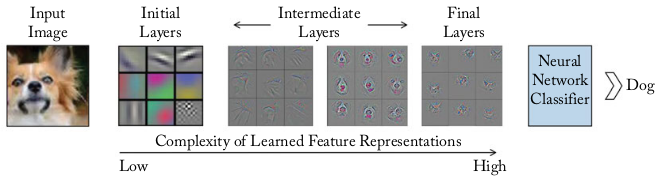
\includegraphics[width=0.9\textwidth]{imgs/camadas-convolucionais}
\label{fig:camadas-convolucionais}
\end{figure}


% Pooling
Uma camada de \emph{pooling} em uma CNN opera em blocos do mapa de características e combina seus atributos através da operação de \emph{max pooling} ou \emph{average pooling}. Esse bloco é deslizado através do mapa de características com um passo definido como \emph{stride}. A operação de \emph{max pooling} retorna o valor máximo dos dados em uma área retangular. Enquanto a operação de \emph{average pooling}, realiza o mesmo processo, porém utiliza a média desses valores. O propósito da camada de \emph{pooling} é, além de diminuir a quantidade de amostras no mapa de características, ajudar a sua representação a se tornar invariante a pequenas mudanças nos dados de entrada \cite{khan, goodfellow}. Uma visualização detalhada dessa operação é demonstrada na Figura \ref{fig:pooling}.

\begin{figure}[h!]
  \centering
  \caption{Visualização da operação de \emph{max pooling} considerando uma região de 2 x 2 com um \emph{stride} igual a 1. Fonte: \cite{khan}.}
  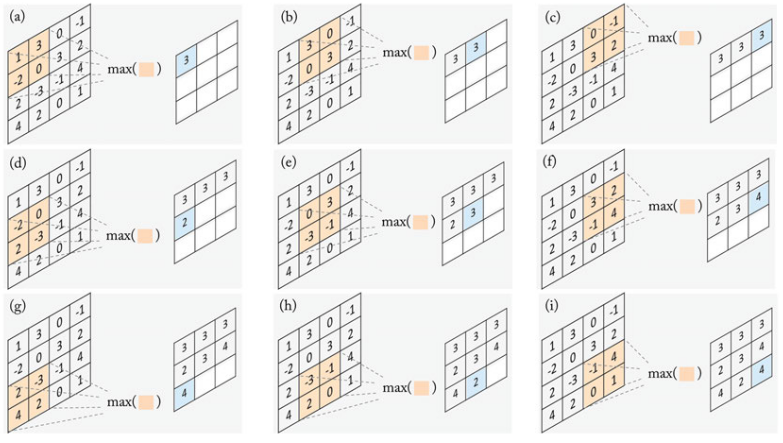
\includegraphics[width=0.8\textwidth]{imgs/pooling}
  \label{fig:pooling}
\end{figure}

% Fully connected layers, camada de saída??

As \emph{Camadas Completamente Conectadas} (FCL, do inglês \emph{Fully Connected Layers}) consideram um conjunto de neurônios completamente conectados aos neurônios da camada anterior, sendo usualmente encontradas no final de uma CNN. Possui a capacidade de separar as variações de classificação que serão retornadas na saída, resumindo os resultados dos vários mapas de características produzidos pela rede \cite{khan}. Na última camada de uma CNN, adota-se geralmente a função de ativação \emph{softmax}, a qual atua escalando as saídas da rede em um vetor de probabilidades, esse processo pode ser muito útil para problemas de classificação \cite{gulli}.

Para prevenir o aprendizado de padrões irrelevantes por um modelo de AM, pode-se articular a quantidade de informações que esse modelo pode armazenar ou adicionar restrições sobre as informações que podem ser armazenadas. Se uma CNN tende a memorizar um pequeno número de padrões, o processo de otimização forçará o foco nos padrões mais proeminentes, que possuem uma chance melhor de gerar uma boa generalização. O processo de evitar o \emph{overfitting} dessa maneira é chamado de \emph{regularização} \cite{chollet}.

O \emph{dropout} é um tipo de regularização muito efetivo e que é usualmente utilizado em CNNs. Consiste na desativação temporária de alguns neurônios durante a fase de treinamento de uma rede. Nesse processo, os neurônios são desativados mediante uma probabilidade $p$, conhecida como \emph{dropout rate}, retornando um valor de saída igual a $0$. Na fase de teste da rede, nenhum neurônio é desativado, ao passo que, como forma de balanceamento devido a quantidade maior de neurônios presentes em comparação à fase de treinamento, os valores de saída das camadas são reduzidos por um fator igual ao \emph{dropout rate} \cite{chollet}. Dessa maneira, pode-se afirmar que o \emph{dropout} ajuda a previnir o \emph{overfitting} ao possibilitar uma forma de combinar diferentes arquiteturas de redes neurais \cite{buduma}. Esta operação pode ser visualizada na Figura \ref{fig:dropout}, na qual os neurônios desativados são demonstrados pelas circunferências com a borda pontilhada.

% Dropout (Pegar imagens sobre Dropout na pagina favoritada )
\begin{figure}[h!]
  \centering
\caption{Processo de aplicação da operação de \emph{dropout}. Os neurônios e ligações desativados estão denotados de forma pontilhada. Fonte: \cite{dsacademy}}
  \subfloat[Arquitetura de uma rede antes da aplicação do \emph{dropout}.\label{subfig:dropout-before}]{%
    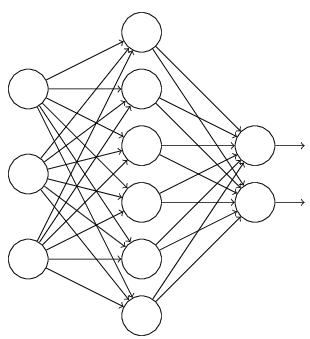
\includegraphics[width=0.4\textwidth]{imgs/dropout-before}
  }
  \hfill
  \subfloat[Arquitetura da rede após a aplicação do \emph{dropout}.\label{subfig:dropout-after}]{%
    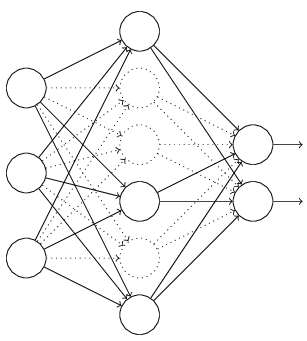
\includegraphics[width=0.4\textwidth]{imgs/dropout-after}
  }
  \label{fig:dropout}
\end{figure}


\added{Uma vez definidos os elementos integrantes das CNNs, estes podem ser compostos de diferentes maneiras para caracterizar a arquitetura de tais redes. Embora a sua utilização possa ser feita de maneira sistemática, algumas organizações de tais camadas já apresentadas na literatura caracterizam arquiteturas canônicas, as quais foram utilizadas em diferentes problemas com um desempenho significativamente positivo. Desta feita, a seção a seguir contempla algumas destas arquiteturas.}

% Arquiteturas canônicas


\subsubsection{Arquiteturas Canônicas de Redes Neurais Convolucionais}
\label{subsubsec:arq-cnns}

Como mencionado anteriormente, o \emph{ImageNet} é uma base de dados que possui mais de 15 milhões de imagens rotuladas manualmente, de alta resolução, separadas em mais de 22 mil categorias \cite{imagenet}. Visando o uso dessa base, tem sido lançando desde 2010 um desafio anual chamado \emph{ImageNet Large Scale Visual Recognition Challenge} (ILSVRC), no qual possui o intuito de aumentar o desempenho das tecnologias em estado da arte para classificação de imagens e detecção e localização de objetos em imagens \cite{sewak}.

Apesar dos conceitos das camadas que compõem as CNNs serem bastante conhecidos e utilizados, ainda é uma atividade de grande dificuldade e responsabilidade propor arquiteturas de redes neurais que executem determinadas tarefas. Portanto, existem diversas arquiteturas canônicas que apresentam um grande desempenho em treinar e executar tarefas de visão computacional, nas quais a grande maioria foi desenvolvida através do desafio ILSVRC. Devido a grande frequência da utilização dessas arquiteturas, a seguir serão apresentados alguns dos seus aspectos mais relevantes.

A primeira das arquiteturas a ser desenvolvida utilizando camadas convolucionais em vez de camadas completamente conectadas convencionais foi a LeNet, proposta por LeCun em 1998 \cite{lecun}. Uma variante dessa arquitetura é a LeNet-5, composta por sete camadas, nas quais cinco dessas possuem pesos ajustáveis e outras duas são compostas por operações de \emph{max pooling}. Esta arquitetura foi aplicada na identificação de dígitos manuscritos, utilizando o conjunto de dados \emph{Modified National Institute of Standards and Technology} (MNIST) como treinamento. \cite{khan}. Na Figura \ref{fig:lenet} é possível visualizar a composição da LeNet-5.

\begin{figure}[h!]
  \centering
  \caption{A arquitetura LeNet-5. Fonte: \cite{khan}.}
  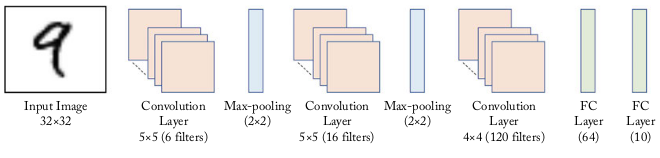
\includegraphics[width=0.8\textwidth]{imgs/lenet5}
  \label{fig:lenet}
\end{figure}

O primeiro modelo em larga escala de CNNs utilizou-se da arquitetura AlexNet, garantindo o primeiro lugar no desafio ILSVRC em 2012 por uma grande margem de diferença dos outros modelos e levando ao ressurgimento da utilização de redes neurais profundas em visão computacional. O uso da função de ativação ReLu após suas oito camadas paramétricas, nas quais as cinco primeiras são convolucionais e as últimas três são completamente conectadas, é um diferencial dessa arquitetura. Operações de \emph{max pooling} são aplicadas após as duas primeiras e a última camada convolucional, ao passo que operações de \emph{dropout} são executadas após as duas primeiras camadas completamente conectadas, acarretando na diminuição do \emph{overfitting} e garantindo uma boa generalização para exemplos não vistos anteriormente \cite{khan}. Apesar de já existirem arquiteturas de CNNs mais eficientes disponíveis, a AlexNet ainda é muito utilizada atualmente, devido a sua estrutura simples e profundidade relativamente menor \cite{sewak}.

A VGGNet é uma das mais populares arquiteturas de CNN desde a sua introdução em 2014 e, mesmo não ganhando o desafio ILSRVC, conseguiu uma taxa de erro de apenas $7.3 \%$. Concebida na Universidade de Oxford, a VGGNet é composta por uma combinação de camadas convolucionais, FCLs, camadas de \emph{pooling} e \emph{dropout}. Esta arquitetura existe em duas versões, a VGG16 e a VGG19, nas quais os números associados aos seus nomes correspondem a sua quantidade de camadas, sem considerar as camadas de \emph{pooling} e \emph{dropout} \cite{khan, sewak}. A VGGNet usa apenas filtros de convolução com uma dimensão de  $3 \times 3$ e as operações de \emph{max pooling} são realizadas através de uma janela de $2 \times 2$ pixeis com um \emph{stride} igual a $2$ \cite{simonyan}.

A arquitetura GoogLeNet, também chamada de Inception, foi desenvolvida pela empresa Google e se tornou a vencedora do desafio ILSRVC de 2014. Seu diferencial em relação às outras arquiteturas foi a combinação não sequencial das suas 22 camadas convolucionais. Como mostrado na Figura \ref{fig:inception-module}, cada camada é executada de forma paralela com outras camadas formando um módulo chamado Inception, que condensa os mapas de características obtido por cada camada e passa como entrada para o próximo bloco Inception encontrado na rede \cite{khan}. Na GoogLeNet, geralmente ocorre o uso de convoluções $1 \times 1$ com a função de ativação ReLu com intuito de diminuir as dimensões do problema antes das dispendiosas convoluções de $3 \times 3$ e $5 \times 5$ \cite{sewak}.

\begin{figure}[h!]
  \centering
  \caption{Exemplo de um módulo Inception da GoogLeNet. Fonte: \cite{khan}.}
  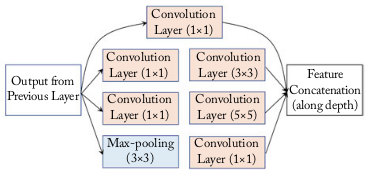
\includegraphics[width=0.6\textwidth]{imgs/inception-module}
  \label{fig:inception-module}
\end{figure}

A Microsoft \emph{Residual Network} (ResNet) foi a CNN vencedora do desafio ILSVRC 2015 com um grande ganho em desempenho, diminuindo a taxa de erro top-5 para apenas $3.6\%$ em comparação à taxa de $6.7\%$ da vencedora do ano anterior, a GoogLeNet. Com o total de 152 camadas, a ResNet deve seu sucesso aos chamados blocos residuais, representado na Figura \ref{fig:residual-block}, no qual as entradas originais são submetidas a uma função de transformação que é conectada diretamente à entrada, chamada de \emph{skip identity connection}. Segundo Khan, uma rede muito profunda sem nenhuma conexão residual obtem uma taxa maior de erro no treinamento e no teste, portanto, as conexões residuais são consideradas fatores importantes para uma melhor classificação de redes neurais profundas \cite{khan}.

\begin{figure}[h!]
  \centering
  \caption{Estrutura de um bloco residual da ResNet. Fonte: \cite{khan}.}
  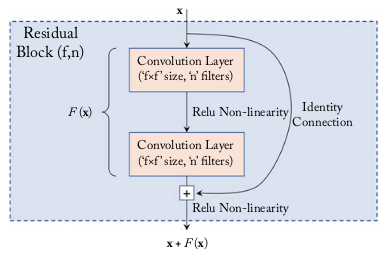
\includegraphics[width=0.6\textwidth]{imgs/residual-block}
  \label{fig:residual-block}
\end{figure}
